\documentclass[conference]{IEEEtran}
\IEEEoverridecommandlockouts
% The preceding line is only needed to identify funding in the first footnote. If that is unneeded, please comment it out.
\usepackage{cite}
\usepackage[portuges,brazil,english]{babel}
\usepackage{amsmath,amssymb,amsfonts}
\usepackage{algorithmic}
\usepackage{graphicx}
\usepackage{textcomp}
\usepackage[ruled,vlined,linesnumbered,portuguese]{algorithm2e}
\usepackage[utf8]{inputenc}
\def\BibTeX{{\rm B\kern-.05em{\sc i\kern-.025em b}\kern-.08em
    T\kern-.1667em\lower.7ex\hbox{E}\kern-.125emX}}
\begin{document}

\title{Trabalho 1 - MC886 Aprendizado de Máquina}

\author{\IEEEauthorblockN{Leo Yuuki Omori Omi}
\IEEEauthorblockA{
138684 \\
leoyuuki@gmail.com}
\and
\IEEEauthorblockN{João Pedro Ramos Lopes}
\IEEEauthorblockA{
139546 \\
jpedrorl@gmail.com}}

\maketitle

\section{Introdução}


Neste trabalho, temos o objetivo de explorar as técnicas de classificação vistas em aula para construir um sistema de reconhecimento de objetos para classificar imagens. Utilizando a Regressão Logística e Redes Neurais, iremos construir vários modelos para classificar imagens do conjunto de dados CIFAR-10.

\section{Regressão Linear}
 
A regressão logística é um método utilizado em Aprendizado de Máquina para classificação. Este método utiliza a função sigmóide para predizer uma probabilidade de uma entrada ser de um determinado conjunto ou não.


\section{Soluções Propostas}
Para uma solução melhor que a base, decidimos por rodar diferentes experimentos em cima dos dados para que pudéssemos achar uma solução boa para o problema. Foram verificadas features que individualmente obtiam menores erros nas predições, graus diferentes para as features, entre outras manipulações dos dados com o objetivo de obter uma predição mais precisa.

\subsection{Solução Base}
Para uma solução base, foi utilizada a regressão linear usando todas as 90 \textit{features} de aúdio diretamente na função de regressão linear do Sickit Learn usando os valores padrões da função. Também foi utilizado como solução base um modelo utilizando múltiplos graus para o polinomio visando a encontrar melhores resultados que a solução com apenas grau 1 para todas as features. 

\subsection{Solução Batch-Gradient}
Neste método, os coeficientes do polinômio são encontrados utilizando um ciclo de aproximações sobre todos os elementos do conjunto de treino até que o resultado atinja convergência. O algoritmo \ref{alg:batch}, disposto em pseudo-código, onde LR é a taxa de aprendizado, apresenta esse modelo.

\begin{algorithm}
		\caption{Pseudo-codigo para gradiente em Batch}
		\label{alg:batch}
		\Inicio{
			\tcp{Inicializacao}
			$coef = [0] * num\_features$ \\
			$intercept = 0$\\
			$iterations = 0$
			
			\Repita{ $iterations < max\_iterations$ }{
			\tcp{ gradiente de cada coeficiente } 
				$i\_grad = 0$
				$c\_grad = [0] * num\_features$\\
				$m = tamanho_conjunto_treino$
				\Para{ cada p no conjunto de treino }{
					$y = p.ano\_esperado$\\
					$h = (y - (calcula\_y(p.valores\_x, coef, intercept)))$\\
					$i\_grad += -(2 / m) * (y - h)$\\					
					$c\_grad += -(2 / m) * p.valores\_x * (y - h)$
				}
				$intercept = intercept - (LR * i\_grad)$\\
				$coef = coef - (lr * c\_grad)$\\
				$iterations = iterations + 1$
			}
		}
	\end{algorithm}
	
\subsection{Solução Stochastic-Gradient}
Neste método, os coeficientes do polinômio são encontrados utilizando um ciclo de aproximações sobre os elementos do conjunto, sendo que o gradiente é calculado sobre cada elemento individualmente, até que o resultado atinja convergência. O algoritmo \ref{alg:stochastic}, disposto em pseudo-código, onde LR é a taxa de aprendizado, apresenta esse modelo.

\begin{algorithm}
		\caption{Pseudo-codigo para gradiente Estocástico}
		\label{alg:stochastic}
		\Inicio{
			\tcp{Inicializacao}
			$coef = [0] * num\_features$ \\
			$intercept = 0$\\
			$iterations = 0$
			
			\Repita{ $iterations < max\_iterations$ }{
				\Para{ cada p no conjunto de treino }{
					\tcp{ gradiente de cada coeficiente } 
					$i\_grad = 0$\\
					$c\_grad = [0] * num\_features$\\
					$y = p.ano\_esperado$\\
					$h = (y - (calcula\_y(p.valores\_x, coef, intercept)))$\\
					$i\_grad += -(y - h)$\\					
					$c\_grad += -p.valores\_x * (y - h)$\\
					$intercept = intercept - (LR * i\_grad)$\\
					$coef = coef - (lr * c\_grad)$				
				
				}
				$iterations = iterations + 1$
			}
		}
	\end{algorithm}	
	
\subsection{Solução Algoritmos Genéticos}
Algoritmos Genéticos se baseam nos conceitos genéticos da biologia evolutiva. Inicialmente é escolhido um conjunto de soluções viáveis denominado população inicial. A cada iteração o algoritmo cruza as soluções de uma dada população, obtendo novas soluções cruzadas, possivelmente realizando mutações, e então seleciona uma população sobrevivente para formar a próxima geração \cite{gendreau2010handbook}. É esperado que a cada geração a população evolua para uma solução mais próxima da solução ótima do problema. O Algoritmo \ref{alg:genetic} apresenta um pseudo-código geral do modelo de Algoritmos Genéticos.

Para a Redução Linear, cada cromossomo contém os valores contínuos dos coeficientes do polinômio de grau 1 e o valor de interceção com o eixo y. 

		\begin{algorithm}
		\caption{Pseudo-código para Algoritmos Genéticos}
		\label{alg:genetic}
		\Inicio{
			\tcp{Inicialização}
			$pais = populacao\_inicial()$ \\
			$filhos = \{\}$\\
			\BlankLine
			\tcp{Evoluir população}
			\Repita{ condicao\_de\_parada}{
				\Repita{ tamanho(filhos) suficiente }{
					\tcp{Geração}
					$cromossomos\_pais = seleciona\_pais(pais)$
					$cromossomo\_filho = crossover(cromossomos\_pais)$
					$mutacoes(cromossomo\_filho)$
					\BlankLine
					\tcp{Seleção}
					\Se { viavel(cromossomo\_filho) }{
						$filhos = filhos \cup {cromossomo\_filho}$
					}
				}
				\BlankLine
				\tcp{Atualiza nova geração}
				$pais = filhos$\\
				$filhos = \{\}$
			}
		}
	\end{algorithm}

\section{Experimentos}
\subsection{Modelos iniciais}
Para o modelo base e de múltiplos graus de regressão linear, utilizamos de \textit{k-fold cross-validation}, com k=5 conjuntos, para verificarmos o funcionamento dos modelos. Para os experimentos, utilizamos estes conjuntos de dados para podermos ver o Erro Quadrático Médio da predição do conjunto de treino e do conjunto de validação para verificarmos se houve \textit{overfitting} (ou \textit{underfitting}). Como medição de precisão antes de utilizar o conjunto de testes, calculamos a média do erro quadrático médio da predição do treino e da validação dentro dos 5 conjuntos da cross-validação.

\subsubsection{Solução Base}
A solução base, que utiliza todas as 90 \textit{features}, obteve um erro quadrático médio de 91.25 para a predição do conjunto de treino e de 91.30, o que já é um resultado consideravelmente bom.

\subsubsection{Solução de múltiplos graus no polinomio}
Para obter uma solução mais complexas com melhores resultados, decidimos utilizar os dados de novas maneiras, e rodamos diferentes experimentos para obter um modelo mais preciso. Um dos primeiros experimentos foi separar os dados de timbre médio, utilizar a regressão linear apenas com estes dados e aumentar o grau do polinômio para todos estes dados para checar se poderíamos obter um erro menor. Ao mesmo tempo, verficamos se havia uma discrepância muito grande entre o erro quadrático médio da predição do conjunto de treino e o erro do conjunto de validação, pois poderia indicar overfitting caso aumentássemos muito o grau do polinômio. O mesmo foi feito então para os dados de covariância do timbre. O intuito de separar os dois tipos de dados, foi a ideia de que um conjunto de dados teria um compartamento similar dentro de dele mesmo, mas teria um comportamento diferente do outro tipo.

Para os dados de timbre médio, até polinômios de grau 7, a discrepância entre os erros não aumentava muito. No entanto, o erro não diminuía muito, e para grau 5 o coeficiente linear resultante foi de 2029, o que e para grau 4 foi de 1968, o que parece ser mais razoável, portanto decidimos por utilizar o timbre médio até o quarto grau no nosso modelo. Para a covariância do timbre, começa a ocorrer uma discrepância entre os erros do conjunto de treino e de validação à partir do quarto grau, portanto utilizamos o terceiro grau.

Para esta solução foi obtido um erro para conjunto de treino de 86.96 e para o conjunto de validação de 87.78. 

\subsection{Busca dentre 3 modelos (Batch vs Stochastic vs GA)}
Buscando obter melhores resultados, foram implementados 3 modelos onde o conjunto de dados foi dividido entre treino (95\%) e validação (5\%). Para calcular a eficiência de um modelo, foi inicialmente utilizado o Erro Quadrático Médio (RMSE) do conjunto de validação.

\subsubsection{Gradientes (Batch e Estocástico)}

Inicialmente, definimos qual {\it Learning Rate} deveríamos colocar para os modelos de gradiente. Para isso, executamos os dois algoritmos para diversos valores. Para valores muito baixos ($< 10^{-3}$) ambos não convergiram, atingindo valores de erro próximos de 2000. Para valores muito altos ($> 1$), os valores encontrados pela função divergiu e o erro tendeu para infinito. Para ambos os algoritmos, a melhor taxa de aprendizado encontrada foi por volta de 0.01, portanto utilizamos esse valor como padrão. 

Definimos a seguir o número de iterações de cada algoritmo. Para isso, plotamos o gráfico de RMSE pelo número de iterações para o algoritmo Batch (figura 1) e para o algoritmo estocástico (figura 2).


\begin{figure}[h!]
	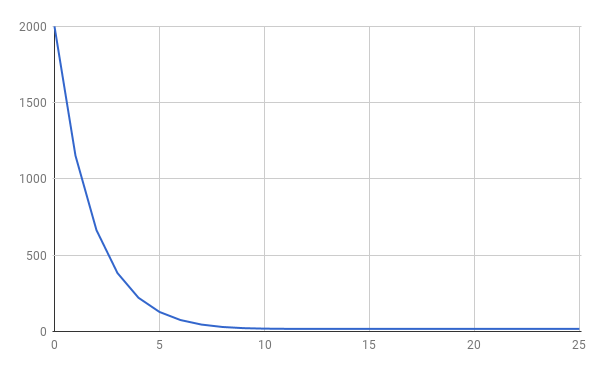
\includegraphics[scale=0.4]{batch.png}
	\caption{Erro x Número de iterações - Modelo Batch}
	\label{fig:batch}
\end{figure}

\begin{figure}[h!]
	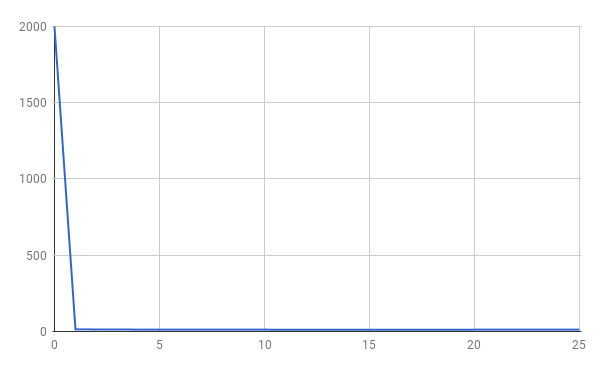
\includegraphics[scale=0.4]{stochastic.png}
	\label{fig:stoc}
	\caption{Erro x Número de iterações - Modelo Estocástico}
\end{figure}

Em seguida, determinamos quais features poderiam estar atrapalhando um melhor desempenho da função gradiente. Então dado o conjunto de dados, iteramos na remoção do elemento cuja a remoção melhore o RMSE do conjunto de testes, parando quando a remoção de qualquer elemento aumentaria o erro. Dessa forma, esse método aponto que das 90 features, as 13 a seguir seriam removidas: [2, 3, 4, 5, 8, 11, 25, 35, 40, 45, 68, 77, 86].
Com a remoção dessas features, o erro para 25 iterações do modelo estocástico foi diminuiu de 12.0169 para 11.7527, e no modelo batch, de 16.9823 para 16.5902.

Assim, definimos encontramos algoritmo final para cada modelo, apresentado resultado de validação 16.4928 para batch e 11.3818 para estocástico com 100 iterações. 

\subsubsection{Genetic Algorithms}
Para o algoritmo genético com parâmetros contínuos \cite{continousgenetics} \cite{continuousgenetics2}, a população inicial foi aleatoriezada, onde cada alelo possui valor no intervalo [-100, 100]. Foi utilizada uma população de tamanho 25, mutação de 20\%. A mutação escolhe um intervalo do gene e randomiza os genes no intervalo [-100, 100]. O crossover escolhe para cada alelo um valor aleatório $\beta$ utilizado como peso para um dos pais, enquanto $1 - \beta$.  O algoritmo genético foi configurado com elitismo 1 (apenas o melhor indivíduo prossegue para a próxima geração) e a seleção de cada pai foi feita com base em um torneio de 4 indivíduos. 

Foi encontrado um erro de 18.3959 depois da execução por 3000s (558 gerações) e um erro de 17.7053 após 11344s (2081 gerações) para o conjunto de treino. O gráfico da figura 3 aponta o desenvolvimento do algoritmo ao longo das gerações. O conjunto de validação da melhor solução apontou erro de 17.6403. 

\begin{figure}[h!]
	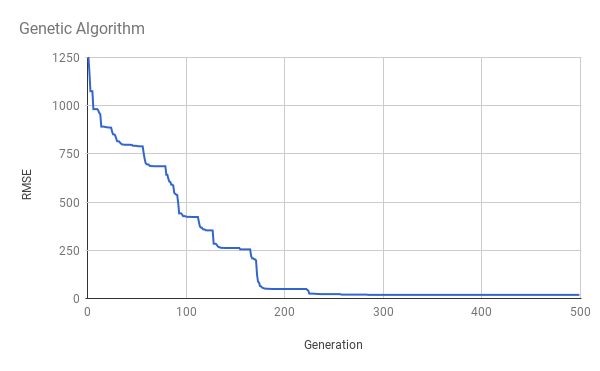
\includegraphics[scale=0.4]{ga.png}
	\label{fig:ga}
	\caption{Desenvolvimento populacional - Algoritmo Genético}
\end{figure}

\subsubsection{Comparação}
Para comparar os três modelos, computamos o RMSE de cada modelo no conjunto de testes. O modelo de gradientes em Batch obteve um erro de 81.14, o modelo estocástico um erro de 45.74 e o algoritmo genético obteve um erro de 25.50. 

Para visualizar melhor os dados, geramos o gráfico dos três modelos computando os erros quadráticos para cada ano, apresentado na figura 4.

\begin{figure}[h!]
	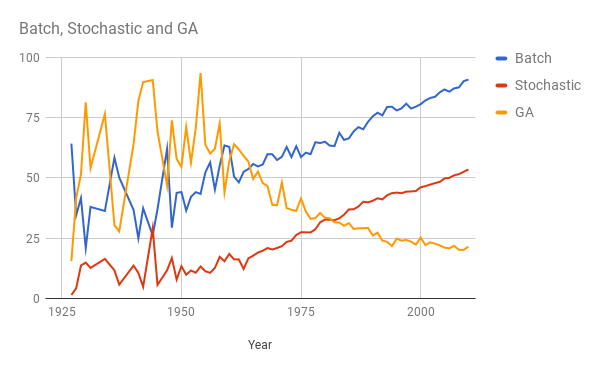
\includegraphics[scale=0.4]{lr_errors.png}
	\label{fig:ga}
	\caption{Erro para cada ano}
\end{figure}


\section{Conclusões}
Sobre os modelos baseados em gradientes, é notável a velocidade de convergência, principalmente no modelo estocástico que obtém erro baixo nas primeiras 5 iterações. Por outro lado, esses modelos necessitam de um fino ajuste da taxa de aprendizado.

É importante apontar que o algoritmo com melhor desempenho final, baseado na meta-heurística de Algoritmos Genéticos, usualmente não é utilizadp para casos contínuos, mas obteve uma boa solução apesar do relativo alto custo de tempo. 

Também é importante notar que os o modelo de GA obteve melhor desempenho para anos com maior número de exemplares do conjunto (próximos do ano 2000), enquanto os outros dois modelos obtiveram melhores desempenhos para anos com um menor número de dados. Esse fato deve ser investigado em trabalhos futuros, visando a encontrar o que levou ao baixo desempenho de modelos comumente aplicados na resolução do problema de Regressão Linear.  


\begin{thebibliography}{00}
\bibitem{linearregression1} Montgomery, D.C., Peck, E.A. and Vining, G.G., 2015. Introduction to linear regression analysis. John Wiley \& Sons.
\bibitem{gendreau2010handbook} Gendreau, M. and Potvin, J.Y., 2010. Handbook of metaheuristics (Vol. 2). New York: Springer.
\bibitem{continousgenetics} Haupt, R.L. and Haupt, S.E., 2004. Practical genetic algorithms. John Wiley \& Sons.
\bibitem{continuousgenetics2} Djurisic, A.B., Elazar, J.M. and Rakic, A.D., 1997. Genetic algorithms for continuous optimization problems-a concept of parameter-space size adjustment. Journal of Physics A: Mathematical and General, 30(22), p.7849.
\end{thebibliography}

\end{document}
